\FloatBarrier
\subsection{Quantum noise features of different topologies}\label{app:QNR}
%\label{subsec:qnft}

Within the design study, there
have been carried out many optimizations of the quantum noise of
different detectors towards different astrophysical sources. In
the following example noise curves are given which are optimized
towards the detection of neutron star binary inspirals, as carried
out in Ref.~\cite{Mueller-Ebhardt2009}. Furthermore, those
examples are attempts to realize the ambitious sensitivity goal of
the Einstein telescope gravitational-wave detector -- in terms of
the quantum noise -- with a single interferometer, where the total
circulating optical power is limited to 3\,MW, the arm length to
10\,km and the test-mass weight to a few hundred kilograms.

The first candidate among the different types of detectors is the
{\bf simple position meter}: here we gather the Michelson
interferometer topology w/o or w/ arm cavities, w/o or w/
power-recycling, w/o or w/ tuned
signal-recycling.
%
\begin{figure}[h]
\centerline{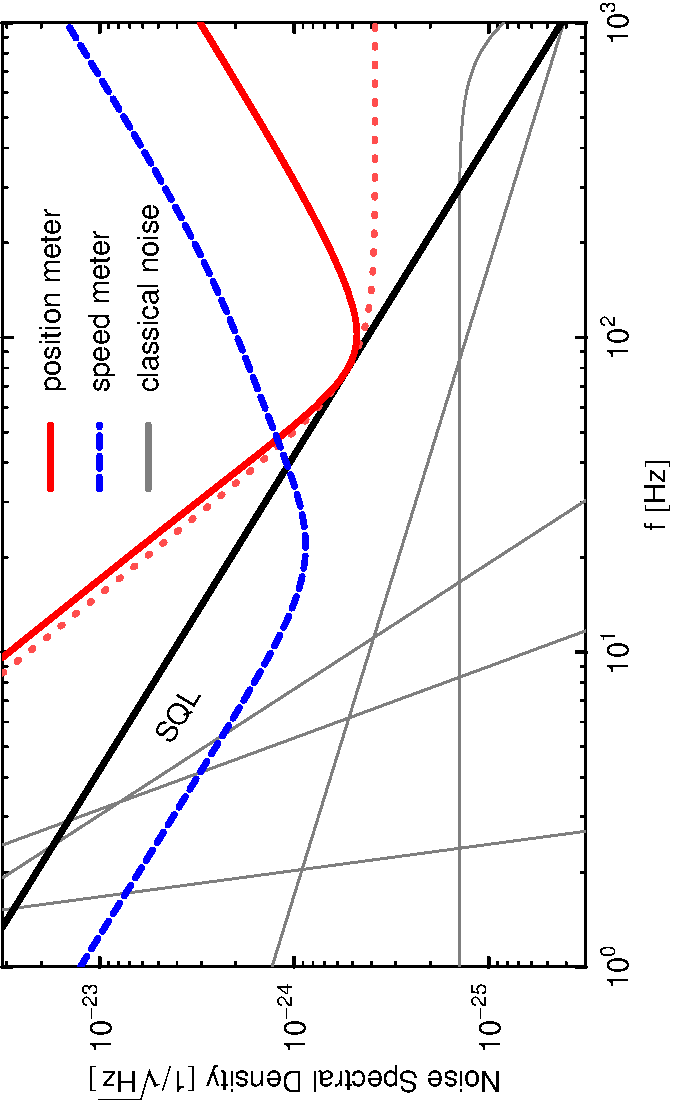
\includegraphics[height=10cm,angle=-90]{./Sec_Optics/ETqnoiseNew.pdf}}
\caption{Example quantum noise spectral densities for position
meter (solid curve), with adiabatically eliminated cavity mode
(dotted curve) and for a speed meter (dashed curve): 10\,km arms;
3\,MW optical power; 120\,kg test-masses. Example noise budget
(gray curves): seismic and gravity gradient noise reduced by a
huge amount compared to advanced detectors; suspension thermal
noise (coating thermal noise) reduced by a factor of 10 (4.5) in
amplitude compared to estimations for Advanced LIGO detector.}
\label{Fig:Michqnoise}
\end{figure}
%
The installation of a power-recycling cavity (by putting an
additional mirror at the bright port of the interferometer) and
the use of cavities in the arms of the interferometer, both
increase the circulating optical power inside the interferometer.
As a consequence, they force up the interaction strength between the laser
field and the test-masses and reduce the shot noise (dominating at
high frequencies) but at the same time increase the
radiation-pressure noise (dominating at low frequencies). From
another point of view (namely when the required circulating
optical power in the arms is fixed) the power-recycling technique
can help to lower the required input power, while using arm
cavities can additionally lower the optical power which has to
pass the beam splitter preventing thermal effects in the
transmissive optics to become a major problem and also minimizing
the bright port / dark port coupling due to the beam splitter
motion~\cite{Harms2004}. The use of arm cavities additionally
increases the signal-susceptibility within the finite bandwidth of
the optical arm resonators, but decreases it above the optical
bandwidth making the shot noise spectral density raise towards
higher frequencies and therefore decreasing the bandwidth of the
gravitational-wave detector. Signal-recycling, as proposed by
Meers~\cite{Meers1988}, can increase the bandwidth of the
gravitational-wave detector by creating an effective bandwidth.
Here an additional mirror, the so-called signal-recycling mirror,
is placed at the dark output port of the interferometer,
reflecting parts of the signal modulation fields back into the
interferometer and forming a signal-recycling cavity either
together with the end mirrors of a simple Michelson interferometer
or with the input mirrors of the interferometer's arm cavities.
The signal becomes recycled which basically means that it is
amplified due to an increase in interaction time between the laser
field and the mirrors. If the signal-recycling cavity is tuned
with respect to the laser frequency, the optical resonator (or the
two coupled optical resonators in a Michelson interferometer with
arm-cavities) have an (effective) bandwidth
which can be greater than the original bandwidth of the
arm-cavities. In such a detector the quantum noise depends mostly
on the optical power circulating in the interferometer, the
bandwidth and length of the cavities and the test-mass weight,
which altogether define the measurement frequency, i.e.\ the
frequency where the quantum noise touches the standard quantum
limit. The strength of the quantum noise is basically shuffled
between high and low frequencies by shifting the measurement
frequency towards higher frequencies. All first generation
laser-interferometric gravitational-wave detectors
(LIGO~\cite{Abbott2009}, VIRGO~\cite{Fiore2002} and
TAMA~\cite{Ando2001}) so far have been constructed as simple
position meters. In Fig.~\ref{Fig:Michqnoise} we see example
quantum noise curves for a simple position meter and the standard
quantum limit for such a detector with 10\,km long arms and
120\,kg test-masses. The quantum noise spectral densities are
plotted for 3\,MW circulating optical power in the arms for a
detector with an effective 50\,Hz cavity-bandwidth (solid curve)
and for a detector with adiabatically eliminated cavity mode
(dotted curve).

Furthermore, the different contributions of an
example classical noise budget for a third generation detector
with classical noise reduction techniques as described within this
design study are additionally adumbrated in
Fig.~\ref{Fig:Michqnoise} and show a big gap between the assumed
classical noise budget and the standard quantum limit. It is
obvious that such a simple position meter would be totally
dominated by the quantum noise, i.e.\ a waste of efforts in the
classical noise reduction, and therefore not suitable to reach the
sensitivity goal of the Einstein Telescope gravitational-wave
detector. For more details refer to e.g.
Ref.~\cite{Mueller-Ebhardt2009} and references therein.

When the signal-recycling cavity is neither resonant nor
anti-resonant with respect to the carrier frequency, the technique
is called detuned signal-recycling. In this case the sensitivity
of the interferometer is enhanced around the (effective) optical
resonance frequency. The signal-recycling technique was already
successfully tested in a 30\,m prototype gravitational-wave
detector~\cite{Heinzel1998,DualRecFreise2000}, in table-top
experiments~\cite{Somiya2005,Miyakawa2006} and has been
implemented into the GEO600 detector~\cite{Grote2004}.
Additionally, the optomechanical coupling in the arm cavities of a
Michelson interferometer with detuned signal-recycling can induce
a restoring force onto the differential motion of the arm-cavities
mirrors---the optical spring effect~\cite{Buonanno2001a}, which
can up-shift the mechanical resonance frequency into the detection
band. We will call such a device an {\bf optical spring
interferometer}~\cite{Buonanno2001a,Buonanno2002,Buonanno2003a,Rehbein2008}.
%
\begin{figure}[h]
\centerline{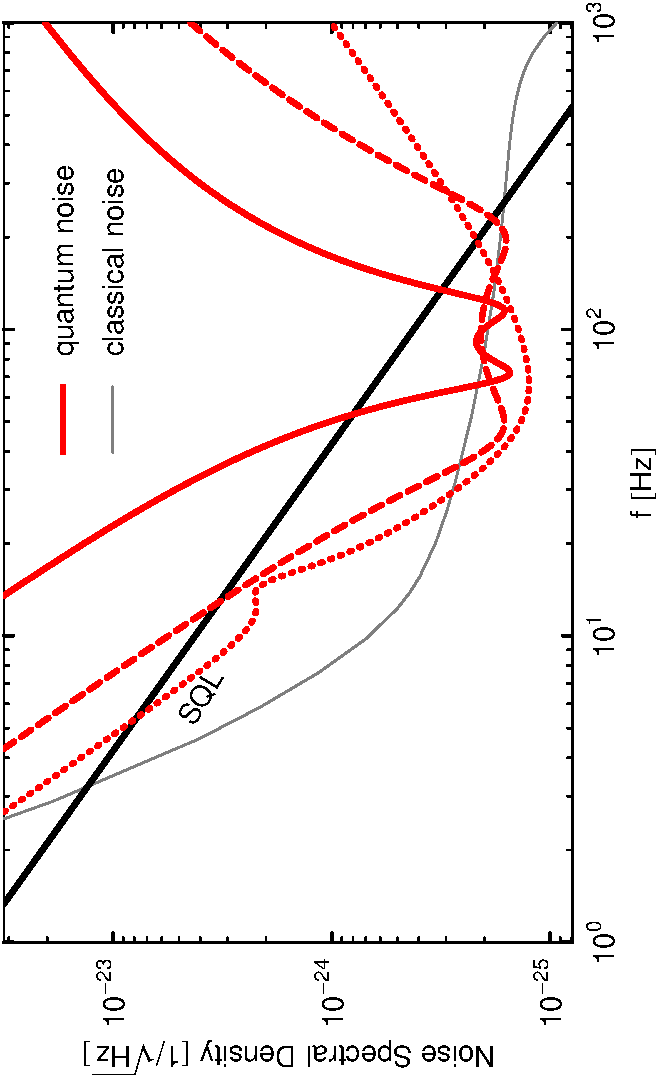
\includegraphics[height=10cm,angle=-90]{./Sec_Optics/EToptMich.pdf}}
\caption{Example quantum noise spectral densities for a Michelson
interferometer with arm cavities (10\,km; 3\,MW optical power;
120\,kg test-mass mirrors) and detuned signal-recycling (136\,Hz
effective detuning; 16\,Hz effective bandwidth; $2\pi/3$ detection
angle)---no input-squeezing (solid curve), no optical loss.
Dashed curve: with 10\,dB frequency-dependent input-squeezing
(208\,Hz effective detuning; 120\,Hz effective bandwidth;
$0.44\,\pi$ detection angle) and 75\,ppm loss in each 10\,km
filter cavity. Dotted curve: variational output with 10\,dB
frequency-independent input-squeezing (4\,Hz effective detuning,
180\,Hz effective bandwidth) and 75\,ppm loss in each 10\,km
filter cavity.} \label{Fig:Michoptqnoise}
\end{figure}
%
Here the sensitivity of the detector is further enhanced around
the second resonance, the optical spring resonance. This
quantum-noise reduction technique belongs to the second group of
methods as defined in Sec.~\ref{sec:qnr}. The optical
spring effect has been demonstrated in a 40\,m prototype
gravitational-wave detector~\cite{Miyakawa2006} and in several
table-top experiments~\cite{Corbitt2007}. Furthermore, the
Advanced LIGO detector~\cite{AdvancedLIGOReference2009} will very likely make use of
the optical spring effect in order to improve the sensitivity. In
Fig.~\ref{Fig:Michoptqnoise} example noise curves for such an
optical spring interferometer are given. For the optical spring
interferometer the optimal quantum noise---optimal for the
specific wave-form of neutron star binary inspirals---becomes
very narrowly peaked around 100\,Hz~\cite{Mueller-Ebhardt2009}. Also
for different astrophysical sources the optimal quantum noise
spectral density is rather narrowband than broadband. Note that
the concept of the optical spring interferometer can be extended
to double optical spring interferometer~\cite{Rehbein2008} or even
multiples optical spring interferometer, where a second (or
multiple) additional frequency-shifted carrier is injected into
the interferometer, creating additional optical springs which can
be used to enhance the sensitivity and additionally stabilize the
optomechanical system within the detection band.

A third detector option is to use an optical {\bf speed
meter}~\cite{Khalili1996}. The idea of using speed meter detectors
was to totally avoid the quantum back-action of the measurement.
At first glance it seems to be very promising to reach this goal
by measuring the speed of the test-masses, because it is usually
proportional to the momentum, which, as a conserved quantity,
cannot introduce any back-action noise. But once the detector
couples to the speed, it has been shown that in this case the
conjugate momentum is actually not proportional to
the speed of the test object~\cite{Khalili2002}. Nevertheless, a speed
meter is able to surpass the standard quantum limit broadbandly by
removing the (frequency-independent) radiation-pressure noise from
the measurement output. The dashed curve in
Fig.~\ref{Fig:Michqnoise} shows a typical example for a quantum
noise curve of a speed meter interferometer---here with 10\,km
long arms, 120\,kg test-masses, 3\,MW circulating optical power in
a 35\,Hz-bandwidth cavity. There exist different proposed designs
of how to realize a speed meter with different topologies: it is
possible to turn a Michelson interferometer topology into a speed
meter by adding a sloshing cavity~\cite{Purdue2002,Purdue2002a} to
the interferometer at the dark output port, where the signal
sloshes back and forth, realizing a time-delayed sensing of the
test-mass position. Another option is to use polarizing optics and
build up a speed meter from a Michelson interferometer topology by
either re-sending the signal into the interferometer multiple
times~\cite{McKenzie2008} or by circulating the light through the
two arms~\cite{Danilishin2004} of the Michelson-like setup. The
most obvious way to realize an optical speed meter, however, is by
using a Sagnac topology with
triangular or rectangular ring cavities in the (folded)
arms~\cite{Chen2003,Mueller-Ebhardt2009a,Eberle2010}. Ignoring the
influence of optical losses, all those different speed meter
realizations have the same quantum noise
performance~\cite{Chen2003} even though they have different
technical advantages and disadvantages.
%
\begin{figure}[h]
\centerline{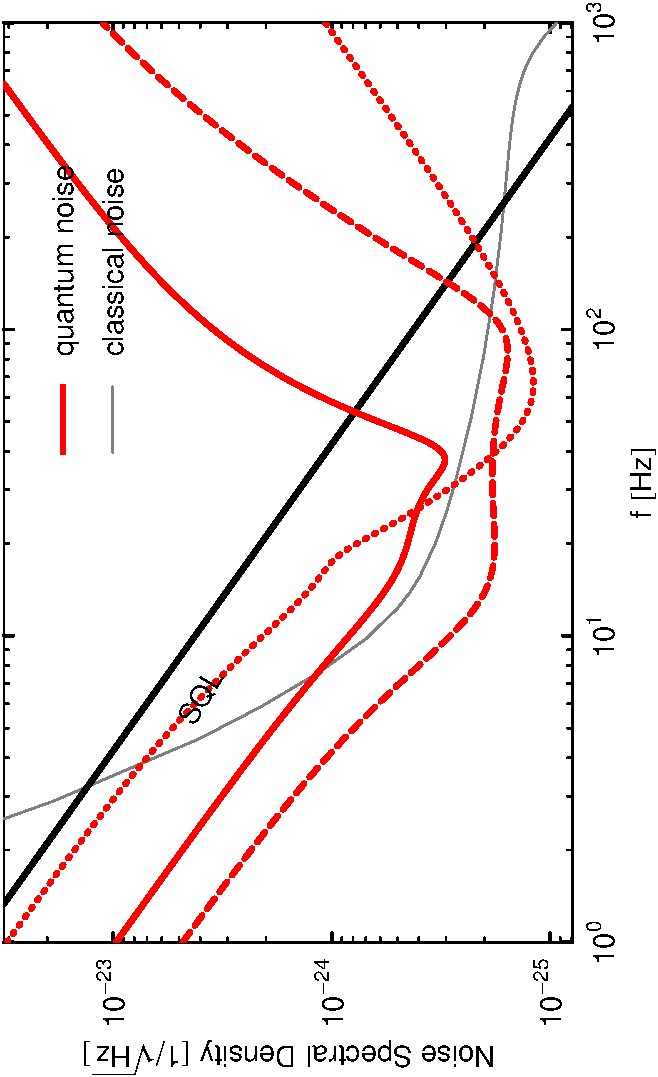
\includegraphics[height=10cm,angle=-90]{./Sec_Optics/EToptSagN.pdf}}
\caption{Example quantum noise spectral densities for a Sagnac
interferometer with ring cavities (10\,km; 3\,MW optical power;
100\,Hz bandwidth; 120\,kg test-mass mirrors) and detuned
signal-recycling (42\,Hz effective detuning; $0.475\,\pi$
detection angle)---no input-squeezing (solid curve), no optical
loss. Dashed curve: with 10\,dB frequency-dependent squeezed input
(150\,Hz bandwidth; 95\,Hz effective detuning; $0.475\,\pi$
detection angle) and 75\,ppm loss in each 10\,km filter cavity.
Dotted curve: variational output with 10\,dB frequency-independent
squeezed input (50\,Hz bandwidth; 0.5\,Hz effective detuning) and
75\,ppm loss in each 10\,km filter cavity.}
\label{Fig:Sagoptqnoise}
\end{figure}
%
The specific quantum-noise feature of a speed meter is that it has
a flat response to the radiation-pressure noise at low
frequencies~\cite{Chen2003}, providing a constant back-action free
detection quadrature. The measurement can therefore be made
shot-noise limited at lower frequencies but with a decreasing
signal transfer~\cite{Sun1996} (cf.\ Fig.~\ref{Fig:Michqnoise}). A
detuned signal-recycling cavity turns a speed meter interferometer
into an {\bf optical inertia
interferometer}~\cite{Mueller-Ebhardt2009a}: the optomechanical
coupling influences the dynamics of the test-masses -- it modifies
their dynamical mass by introducing an optical inertia. In
Fig.~\ref{Fig:Sagoptqnoise} we see the quantum noise of a
signal-recycled Sagnac interferometer, which provides high
sensitivity mainly in the low-frequency regime, due to the speed
meter effect, while the detuned signal-recycling broadens the
sensitivity curve by opening it a little more to the
high-frequency regime~\cite{Mueller-Ebhardt2009}. Note that the
optical inertia can become in principle even negative and then can
cancel the mechanical inertia. The hope is that in this way one
can create a test object which has a high resonance-type
mechanical susceptibility in a broad frequency band. Such a
situation can also be found in the double optical spring
interferometer, by exploiting the frequency dependence of the two
optical springs~\cite{Khalilia}.

Finally, the last option for the main interferometer, which we
want to review here, the {\bf optical
transducer}~\cite{Braginsky1996,Braginsky1997,Khalili2002a,Rehbein2007},
is totally different compared to the others in terms of the
readout method: the idea of such schemes is not to measure the
phase shift of the laser field via monitoring the outgoing
modulations fields at the dark port of an interferometer but to
measure the redistribution of optical energy directly inside an
interferometer by converting the gravitational-wave strain via
radiation pressure into real mirror motion. This motion should
then be sensed by an additional highly sensitive local meter. The
overall sensitivity to gravitational waves for such a transducer
scheme depends not only on the transducer ability of the main
interferometer but also on the sensitivity of the local meter.
Several optical realizations have been proposed: the initial idea
was to construct an optical bar, as an optical analog to an
mechanical bar resonator. Later this topology was extended to the
optical lever scheme~\cite{Khalili2002a}, where the interaction
strength is enhanced by the use of arm cavities. Furthermore, it
had been realized before that also a detuned signal-recycled
Michelson interferometer with arm cavities effectively functions
as an optical bar at low frequencies, where the gravitational-wave
strain is converted into mirror motion of the input mirrors of the
arm cavities. In this case even the realization of a local meter
is straightforward: a second frequency-shifted carrier can be
inserted into the interferometer, which is anti-resonant in the
arm cavities, and therefore forming a small interferometer with
the arm-cavity input mirrors as its end mirrors. This local
readout scheme~\cite{Rehbein2007} is a combination of an optical
bar interferometer and a optical spring interferometer, where the
two outputs can be combined in an ideal way to enhance the
sensitivity at lower frequencies (optical bar) and simultaneously
at higher frequencies (detuned signal-recycled Michelson).

All these different main interferometer detectors can be equipped
with a technique which is usually called {\bf input-squeezing}.
The use of squeezed states of light for improving the sensitivity
of gravitational-wave detectors was first proposed in 1981 by
Caves~\cite{Caves1981}. He showed that the quantum noise limited
sensitivity in a shot noise dominated interferometer can be
enhanced by the injection of broadband (frequency-independent)
squeezed fields into the interferometers signal port. Accordingly
at a point, where the interferometer performance will be limited
by the amount of the achievable circulating light power and the
thermal load in its optics squeezed field injection can be used to
either relax the high power requirement or increase the
sensitivity further. The reduction of shot noise by the aid of
squeezing was later experimentally shown in
Refs.~\cite{Xiao1987,Grangier1987,McKenzie2002} (cf.\ Sec.~\ref{subsec:QNRsqz}).
However, at first view the enhancement of an interferometers
sensitivity with frequency independent squeezing (squeezed light
with a fixed quadrature angle) can only be achieved in a certain
frequency range. This is a direct consequence of the Heisenberg
uncertainty principle. Considering a simple position meter, the
quantum noise in its phase quadrature (shot noise) can be reduced
by the amount of squeezing. Unfortunately, the quantum noise in
the amplitude quadrature (radiation pressure noise) will be
increased by the same amount enhancing the noise at low
frequencies. Later it was revealed by Unruh~\cite{Unruh1982} and
others~\cite{Yuen1983,Pace1993,Jaekel1990} that squeezed field
injection with frequency dependent squeezing angle allows an
overall quantum noise reduction including the radiation pressure
noise. Motivated by the work of Unruh and Jackel~\&~Reynaud the
use of additional input and output optics---namely filter
cavities---was proposed by Kimble~\textit{et al.}~\cite{KLMTV}.
Applying these filters (commonly referred to as Kimble-filters)
converts a conventional interferometer into a broadband quantum
non-demolition interferometer (cf. Sec.~\ref{sec:filtercavities}).
The filters allow the preparation of squeezed states providing a frequency-dependent
squeezed quadrature which is adapted to the interferometers
quadrature rotation. The injection of such a prepared squeezed
state leads to a quantum noise reduction over the entire detection
band. The investigation of Kimble~\textit{et al.} was restricted
to simple position meters. It was shown by Harms~\textit{et
al.}~\cite{OpticalSpringHarms2003} and
Buonanno~\&~Chen~\cite{Buonanno2004} that such filters applied to
optical spring interferometers also allow a broadband quantum
noise reduction by squeezed light. Unfortunately, quite generally
two low-loss, narrow-bandwidth, and therefore long-baseline
optical filter cavities are necessary to prepare the squeezed
states in an optimum way.  The generation of frequency-dependent
squeezing utilizing one filter cavity was experimentally
characterized by Chelkowski~\textit{et al.}~\cite{Chelkowski2005}
followed by the shot noise reduction of a table-top dual-recycled
Michelson interferometer demonstrated by Vahlbruch~\textit{et
al.}~\cite{Vahlbruch2005}. Another way to achieve an enhancement
in the high frequency range without drastically worsen the low
frequency sensitivity by avoiding the use of multiple long
base-line filter cavities was proposed by Corbitt~\textit{et
al.}~\cite{Corbitt2004}. Here, the use of a tuned Fabry-Perot
cavity with two partly transparent mirrors was suggested acting
has high-pass filters (termed amplitude filters within this
context) for the squeezed field. In reflection of this filter
cavity the squeezing at sideband frequencies beyond the filter
cavity bandwidth is preserved whereas at low frequencies the
squeezing is lost and replaced by ordinary vacuum noise. Since any
optical loss of the filters mainly affects the transmitted part,
the baseline of the filters can be chosen comparatively small. It
has already been realized quite early that there is a transition
region between the reduced noise at high frequencies and the
non-increased noise at low frequencies, were the sensitivity is
degraded. Later, this degradation was explained by information
loss at the end mirror of the filter cavity and an additional
homodyne detection was proposed to capture this
information~\cite{Khalili2008}. Furthermore, it has been proposed
to inject additional squeezed vacuum though the filter cavity end
mirror and thus suppress also the low-frequency
radiation-pressure noise~\cite{Khalili2009}. However, these
techniques are more useful for simple position meters and are
intended to be installed as a low-cost add-on during the life
cycle of the second generation detectors~\cite{Khalili}, since the
rotation of the squeezing ellipse around the optical resonance of
optical spring interferometers cannot be compensated by these
filters leading to a deceased sensitivity which can be even below
that of the interferometer without input-squeezing. For speed meter
interferometer the quantum noise can be reduced by input-squeezing
analogously to a position meter with filter
cavities~\cite{Purdue2002a}. But here it is also possible to
achieve an enhancement at lower frequencies without drastically
worsen the high frequency sensitivity avoiding the use of filter
cavities~\cite{Eberle2010}. Furthermore, it has been
experimentally verified that the shot-noise limited sensitivity of
a zero-area Sagnac interferometer can be enhanced by
input-squeezing~\cite{Eberle2010}. In Fig.~\ref{Fig:Michoptqnoise}
and Fig.~\ref{Fig:Sagoptqnoise} one finds examples of quantum
noise spectral densities (dashed curves) for the optical spring and
speed meter interferometer with frequency-dependent input
squeezing in the ideal case of no optical loss.

Additionally, all main interferometer detectors can be equipped
with a balanced homodyne detection and with the {\bf
variational-output} technique, which was invented conceptually in
the early 1990s by Vyatchanin, Matsko and
Zubova~\cite{Vyatchanin1993,Vyatchanin1995} and later
substantiated by Kimble~\textit{et al.}~\cite{KLMTV}. Here filter
cavities are used to make the quadrature angle of the detected
output field frequency dependent and therefore realize a broadband
evasion of the radiation-pressure noise. Even though the most
efficient combination of frequency-dependent input-squeezing and
variational-output for the optical spring interferometer cannot be
realized with Kimble-filters, different semi-optimal configuration
have been found~\cite{Buonanno2004}. Especially at low
frequencies, variational output with frequency-independent
input-squeezing can in principle improve the sensitivity much more
than frequency-dependent input-squeezing, but on the other hand
optical losses in the filter cavities for the variational-output
become even more severe~\cite{KLMTV,Chen2010}. When the
radiation-pressure noise is strong, it is required to bring enough
of the quadrature without signal-content into the output in order
to cancel the radiation-pressure noise and this introduces
significantly higher noise due to optical losses. Moreover,
optical losses in the filters remove parts at low
frequencies of the already weak signal from the output. In
Fig.~\ref{Fig:Michoptqnoise} and Fig.~\ref{Fig:Sagoptqnoise} there
are examples for quantum noise spectral densities (dotted curves)
of variational readout interferometers in the ideal case of no
optical loss given. For more details refer to
Ref.~\cite{Mueller-Ebhardt2009}. 